\chapter{Testování}
%TODO mozna neco z testovani zaradit do sekce realizace. predevsim nejake promerovani parametru? a tady nechat jen zasadni info o dulezitych testech
\section{Napájení}
% TODO V2 rozbehove sekvence celeho zarizeni  !!
% TODO V2 stailita 1V2ANA 1V2DIG pro Timepix2 !!
Na základní desce jsou generované celkem 3 napájecí úrovně z +5V externího napájení přes USB, jak bylo uvedeno v sekci \ref{napajeni}. A to napájecí úrovně +1.2 V, +2.5 V a +3.3 V. Zvlnění výstupního napětí bylo poté vždy měřeno na výstupu každého spínaného regulátoru se snahou vytvoření co nejkratší zemní smyčky mezi měřícím bodem a připojenou zemí osciloskopu. Měření nebylo ve všech případech s ohledem na velikost zemní smyčky ideální vzhledem k zapojení ve kterém je realizováno vyčítací rozhraní a to tedy v zapojení, kdy je deska s Timepix 2 nad základí deskou a tedy není možné se připojit sondou osciloskopu na vrchní stranu základní desky. I s ohledem na zmíněné problémy byly naměřeny tyto průběhy \ref{fig:napeti}. Kde CH3 je +2.5 V, CH2 +3.3V a CH1 poté +1.2 V.
\begin{figure}[h!]
	\centering
	\captionsetup{justification=centering}
	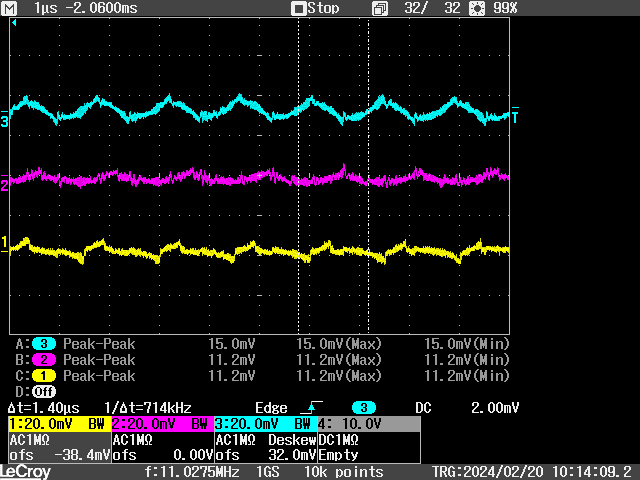
\includegraphics[scale=0.40]{./Mereni/ripple 3V3 - CH2 & 2V5 - CH3 & 1V2 - CH1, 2x 47uF.png}
	\caption{Zvlnění napětí výstupních napětí +2.5V, +3.3 V a +1.2 V } 
	\label{fig:napeti}
\end{figure}
Stabilní stejnosměrné hodnoty výše uvedených napájecích úrovní je možné vidět na obrázku 
\begin{figure}[h!]
	\centering
	\captionsetup{justification=centering}
	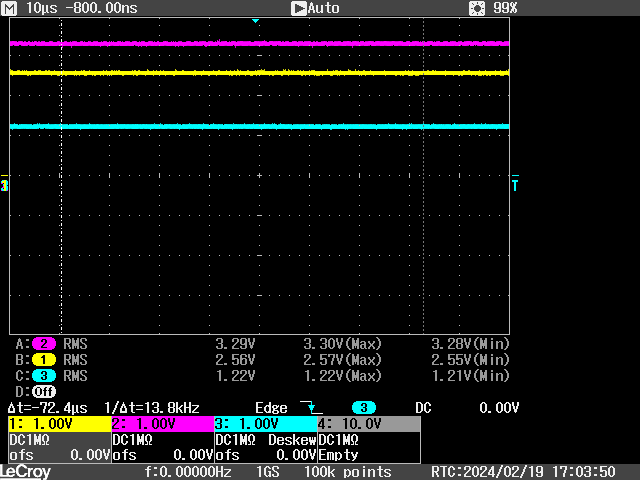
\includegraphics[scale=0.40]{./Mereni/vout 3V3 & 2V5 & 1V2.png}
	\caption{Stjenosměrné úrovně výstupních napětí spínaných regulátorů na základní desce \ref{zakladni deska}} 
	\label{fig:urovne}
\end{figure}

\section{Vysokonapěťový zdroj}
% Nastaveni VN zdroje
%todo Stabilita pro x napeti ? , Zavislost hex na real value
 
\section{Měření teploty}
Typ senzoru který byl pro tuto práci vybrán pro měření teploty na desce s Timepix 2 byl podrobně popsán v části \ref{Mereni teploty}. Pokud dojde k uživatelskému příkazu, který požaduje informaci o teplotě, následuje proces vyčtení teploty ze senzoru, který je zjednodušeně popsán diagramem na obrázku \ref{fig:diagram}.
\begin{figure}[h!]
	\centering
	\captionsetup{justification=centering}
	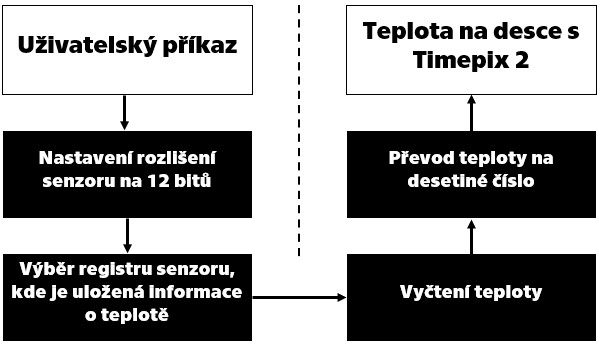
\includegraphics[scale=0.50]{teplota diagram.jpg}
	\caption{Diagram průběhu vyčtení teploty ze senzoru TMP 100 na desce s Timepix 2} 
	\label{fig:diagram}
\end{figure}
% TODO výpis z Terminalu, jeste lepe z TrackLabu
% TODO promereni teploty s mechanikou ??

\section{Komunikační rozhraní s Timepix 2}		% promřování logických urovni komunkikace, rychlosti atd..
%todo logicke urovne SLVS, rychlosti komunikace -> need V2. MCLOCK..

\section{Digitální test Timepix 2} %popis prubehu a vysledku
	\subsection{Vyčtení chip ID}
	\subsection{Vyčtení a zapsání pixelových matic}
\section{USB komunikace}s
%todo, dokumentace funkčnosti... -> VCM, pak UDP pres USB

\section{Měření spotřeby}
%todo spotreba, bez chipu, s chipem, zavislosti?
	\subsection{Porovnání spotřeby} % TODO nebo jen uvest parametry?
	
\section{Dosažené parametry}
% TODO shrnuti nosazenych parametru namerenych vyse